\documentclass{standalone}
\usepackage{tikz}
\usepackage{amsmath}
\usetikzlibrary{automata, positioning, arrows.meta}

\begin{document}
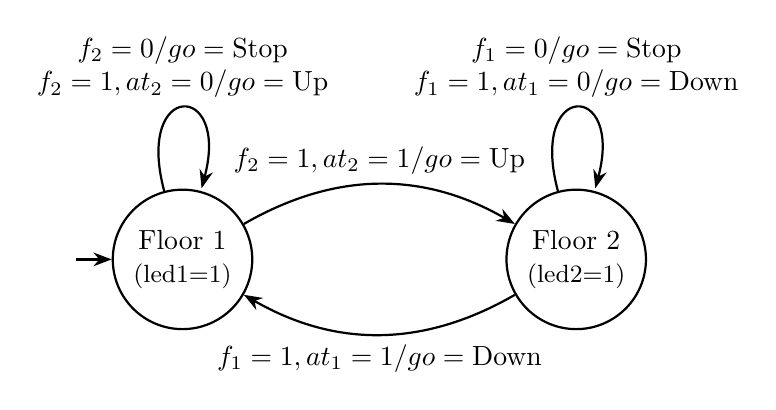
\begin{tikzpicture}[>=Stealth, node distance=5cm, on grid, auto, thick, initial text=]
    \node[state, initial, align=center] (F1) {Floor 1 \\ \small{(led1=1)}};
    \node[state, align=center] (F2) [right=of F1] {Floor 2 \\ \small{(led2=1)}};

    \path[->]
        (F1) edge [loop above] node [align=center] {$f_2=0 / go=\text{Stop}$ \\ $f_2=1, at_2=0 / go=\text{Up}$} (F1)
             edge [bend left]  node [align=center] {$f_2=1, at_2=1 / go=\text{Up}$} (F2)
        (F2) edge [loop above] node [align=center] {$f_1=0 / go=\text{Stop}$ \\ $f_1=1, at_1=0 / go=\text{Down}$} (F2)
             edge [bend left]  node [align=center] {$f_1=1, at_1=1 / go=\text{Down}$} (F1);
\end{tikzpicture}
\end{document}
